\section{Real-time Communication}

%% 
%% Leave first page empty
\thispagestyle{empty}

Real-time Communication can be defined as any mode of communication where users can exchange information and media with low latency, real-time aspect of it can be defined as live. The purpose of RTC is widely seen as a way to intercommunicate between people or software. This can be done in a two-way scenario where data is transmitted between both sides, being both users receivers and senders, or in a one-way configuration with one unique source of data and one or multiple receivers. In the first configuration latency is very important in order to achieve good common communication between both users whereas the second scenario can tolerate some latency in the link but data transmission must be continue. In two-way communication data can be transmitted using multiple technologies, the topologies used can be either peer-to-peer or using a centralized relay. Some other ways of transmitting data include multicast or broadcast.

In broadcast and multicast mode data is transferred to multiple peers in a network but does not require to be real time in most cases.

\begin{figure}[h]
  \centering
    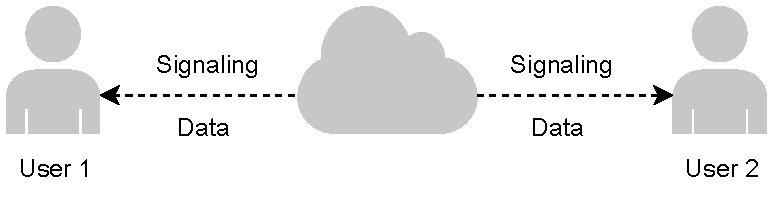
\includegraphics[width=1\textwidth]{./figures/P2P.pdf}
      \caption[Real time communication between two users over the Internet]{Real time communication between two users over the Internet.}
	\label{fig:RTC}
\end{figure}

Figure~\ref{fig:RTC} describes an RTC scenario for two users, the technology that provide the communication may differ in each situation but the goal is always the same. RTC has two important characteristics that are always common in all technologies, there must be a signaling or agreement between the two entities, either with the central node or with the other user. This part is used by the protocols to check the capabilities of the two entities before proceeding to send the media. In this part, codec agreement and keep-alive methods are decided at the same time as all the multiple features that will be enabled in the new session, making it crucial to configure the media and data to be transmitted.

On the other hand, once signaling is done data can be sent to the receiver, this data may include media (audio or video) and data. This transmission may require also some extra signaling messages to be exchanged in order to maintain the link or adapt the constraints to the actual network conditions. 

RTC can be either over the Internet or using traditional techniques, some of them are: telephony, mobile phone communication, radio, instant messaging (IM) \nomenclature{IM}{Instant Messaging}, Voice over IP (VoIP) \nomenclature{VoIP}{Voice over IP},  Video and Voice over IP (VVoIP) \nomenclature{VVoIP}{Video and Voice over IP}, Internet Relay Chat (IRC) \nomenclature{IRC}{Internet Relay Chat} and videoconferencing. 

All the previous ways of communication work in real time, logically they work using Figure~\ref{fig:RTC} topology but with different kind of protocols. In this thesis we will manly work with Internet RTC using media and data.
%Web Real-Time Communication is a technology that builds P2P applications by using a defined JavaScript API. The first announcement went public in a WG of the World Wide Web Consortium (W3C) in May 2011~\cite{webrtcW3cgroup} and started the official mailing list in April 2011~\cite{welcomeW3C}. During the first stage of discussion, the main goal was to define a public draft for the version 1 API implementation and a route timeline with the goal to publish the first version by March 2013. The first public draft of W3C came public the 27th of October 2011~\cite{originalW3Cdraft}. During this first W3C draft, only media (audio and video) could be sent over the network to other peers, it is focused in the way browsers are able to access the media devices without using any plugin or external software.
%
%Alongside to the W3C working group, the WebRTC project also joined the IETF with a WG in May 2011~\cite{webrtcIETFgroup} with the first public announcement charter done the 3th of May 2011~\cite{webrtcIETFcharter}. Milestones of the WG initially marked December 2011 as deadline to provide the information and elements required to the W3C for the API design input. On the other side, the main goals of the WG covered the definition of the communication model, session management, security, NAT traversal solution, media formats, codec agreement and data transport~\cite{webrtcIETFcharter}.
%
%One  of the most important steps during the process of standardization came the 1st of June 2011 when Google publicly released the source code of their API implementation~\cite{haraldpublicWebRTC}. 
%
%During all this period both WGs have been working alongside to provide a reliable solution to enable cross-platform applications to perform media and data P2P transfer over the browser in a plugin-free environment. The first final version of the WebRTC API is to be published at the end of 2013.
%
%Some alternatives are available to the WebRTC concept, considering the global architecture of WebRTC, Session Initiation Protocol (SIP) and Secure Real-Time Media Flow Protocol (RTMFP) are similar approaches to the same solution.

\subsection{Session Initiation Protocol (SIP) \nomenclature{SIP}{Session Initiation Protocol}}

SIP allows communication between two different users with audio/video support in real-time. SIP final Request for Comments (RFC) \nomenclature{RFC}{Request for Comments} was published in June 2004, this document describes the original functionalities and mechanisms of SIP~\cite{sipRFC}. From an overview perspective, SIP is an application-layer control protocol for multimedia sessions which can establish, maintain and terminate media sessions. During the development of the standard different new functionalities were added to the drafts such as conferencing and the possibility of adding/removing media from existing sessions. 

%SIP differentiates from RTMFP/WebRTC by locating the end user to be used for communication, this feature allows SIP to be closely related to traditional PSTN networks as it allow cross-domain communication which is not possible when using RTMFP/WebRTC. SIP is not a complete toolkit for communications. <<-- SUMMARY OF RTC

This protocol work alongside with other existing technologies such as Real-time Transport Protocol (RTP) \nomenclature{RTP}{Real-time Transport Protocol}, Session Description Protocol (SDP) \nomenclature{SDP}{Session Description Protocol} and Media Gateway Control Protocol (MEGACO) \nomenclature{MEGACO}{Media Gateway Control Protocol}. Using SDP for the session negotiation between the end-points and RTP for the media transport, all these protocols are widely used in other technologies and usually provide legacy for older devices and outdated versions. Meanwhile SIP can locate and deliver a message to a user, SDP can provide the required information for the session establishment and RTP can transport the data.

\begin{figure}[h]
  \centering
    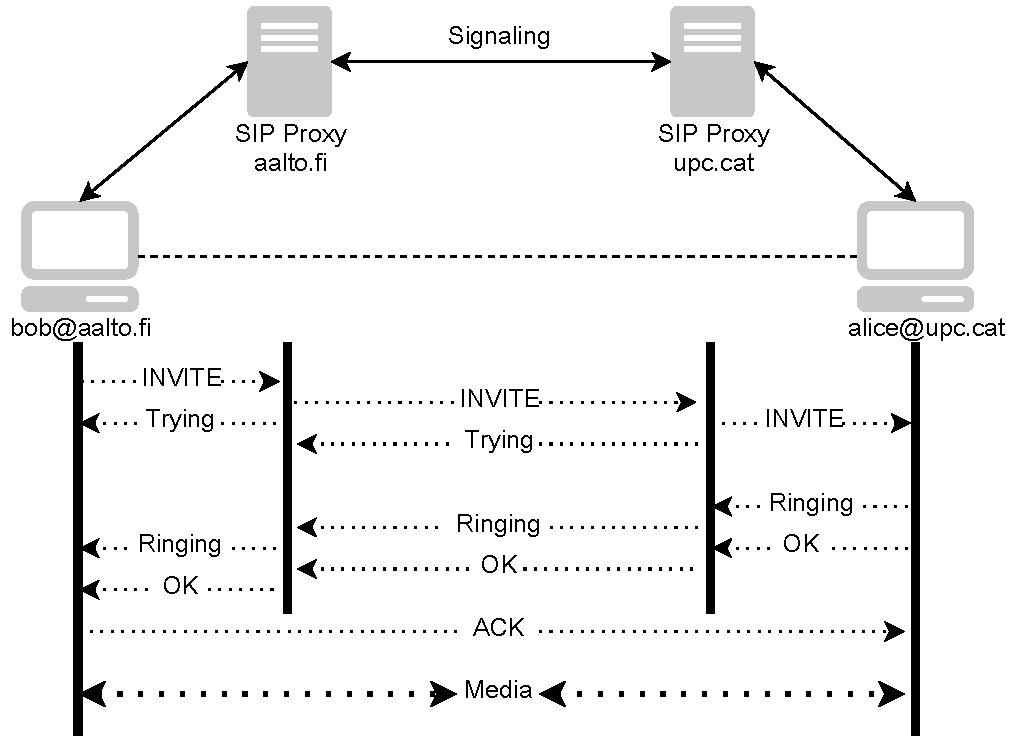
\includegraphics[width=1\textwidth]{./figures/SIParchitecture.pdf}
      \caption[SIP architecture for end-to-end signaling]{SIP architecture for end-to-end signaling.}
	\label{fig:SIParchitecture}
\end{figure}

SIP architecture relies in a trapezoid form where the Domain Name System (DNS) \nomenclature{DNS}{Domain Name System} is used to locate the other peers of the system. Once that peer is located and session is negotiated, media flows peer-to-peer directly to the endpoint. In order to build this system different agents are needed, SIP Proxies, SIP Redirect and SIP Registrar. SIP Proxies transmit the SDP and SIP messages from one peer to the other to establish communication (Figure~\ref{fig:SIParchitecture}). SIP Registrar are the machines that collect and save all the user information from the end points.

DNS provides the IP address for both proxy servers and allows the messages to be exchanged between both peers, SIP uses the following three-way handshake: INVITE, 200OK and ACK. Those messages carry the SDP data inside in an object format, when ray@upc.cat receives the INVITE message from bob@aalto.fi builds the 200OK response carrying the SDP object that provides compatibility check between both peers and which options and codecs to use. SIP provides some more messages to update the already existing session or to close them. The media transport is done using RTP and RTCP using User Datagram Protocol (UDP) \nomenclature{UDP}{User Datagram Protocol}~\cite{sipRFC}.

SIP is a pure VoIP confederated technology that helped the community to learn about real-time P2P communication.

\subsection{Real Time Media Flow Protocol (RTMFP) \nomenclature{RTMFP}{Real Time Media Flow Protocol} and Adobe Flash}

RTMFP and Adobe Flash are proprietary technologies provided by Adobe, both services work together to provide multimedia and RTC between users.

Adobe Flash is a multimedia software that uses a plugin to work on top of the browser, it is used to build multimedia experiences for end users such as graphics, animation, games and Rich Internet Applications (RIA) \nomenclature{RIA}{Rich Internet Application}. It is widely used to stream video or audio in web applications, in order to reproduce this content we need to install Adobe Flash plugin in our computer. It also uses a different programming language that do not comply with any standards called JavaScript Flash Language (JSFL) \nomenclature{JSFL}{JavaScript Flash Language} and ActionStript. RTMFP and Adobe Flash require a plugin to work with any device, this obliges the user to install extra software that is not included in the browser, these two technologies are not standardized and are difficult to enable in some mobile devices. Adobe Flash Player is available in most platforms except iOS devices and reaches about 98\% of all internet-enabled desktop devices. This plugin allows developers to access media streams from external devices such as cameras and microphones to be used along with RTMFP.

RTMFP uses Adobe Flash to provide media and data transfer between two end points. This system works over UDP~\cite{rtmfpDraft}. RTMFP provides a full suite of methods and functions that allow the browser to access the necessary mechanisms to run real-time media communication, those methods are included into the plugin that must be installed prior usage. RTMFP is a private and licensed protocol. It also handles congestion control on the packets and NAT transversal issues. One of the biggest differences is that, compared with SIP, RTMFP does not provide inter-domain connectivity and both peers must be in the same working domain to be able to communicate. This protocol is implemented by using Flash Player, Adobe Integrated Runtime (AIR) and Adobe Media Server (AMS) \nomenclature{AMS}{Adobe Media Server}~\cite{rtmfpDraft}. 

Media transfer in this protocol is encrypted, this issue has been addressed clearly in RTMFP by using proprietary algorithms and different encryption methods. The RTMFP architecture is similar to WebRTC concept, it also allows reconnection in case of connectivity issues and works by multiplexing different media streams over the same media channel when handling conferences or multiple streams. For the signaling part Adobe uses a service called Cirrus (Figure~\ref{fig:RTMFParchitecture}), this service allows architectures such as: end-to-end, many-to-many and multicast~\cite{cirrusFAQ}.
 
 \begin{figure}[h]
  \centering
    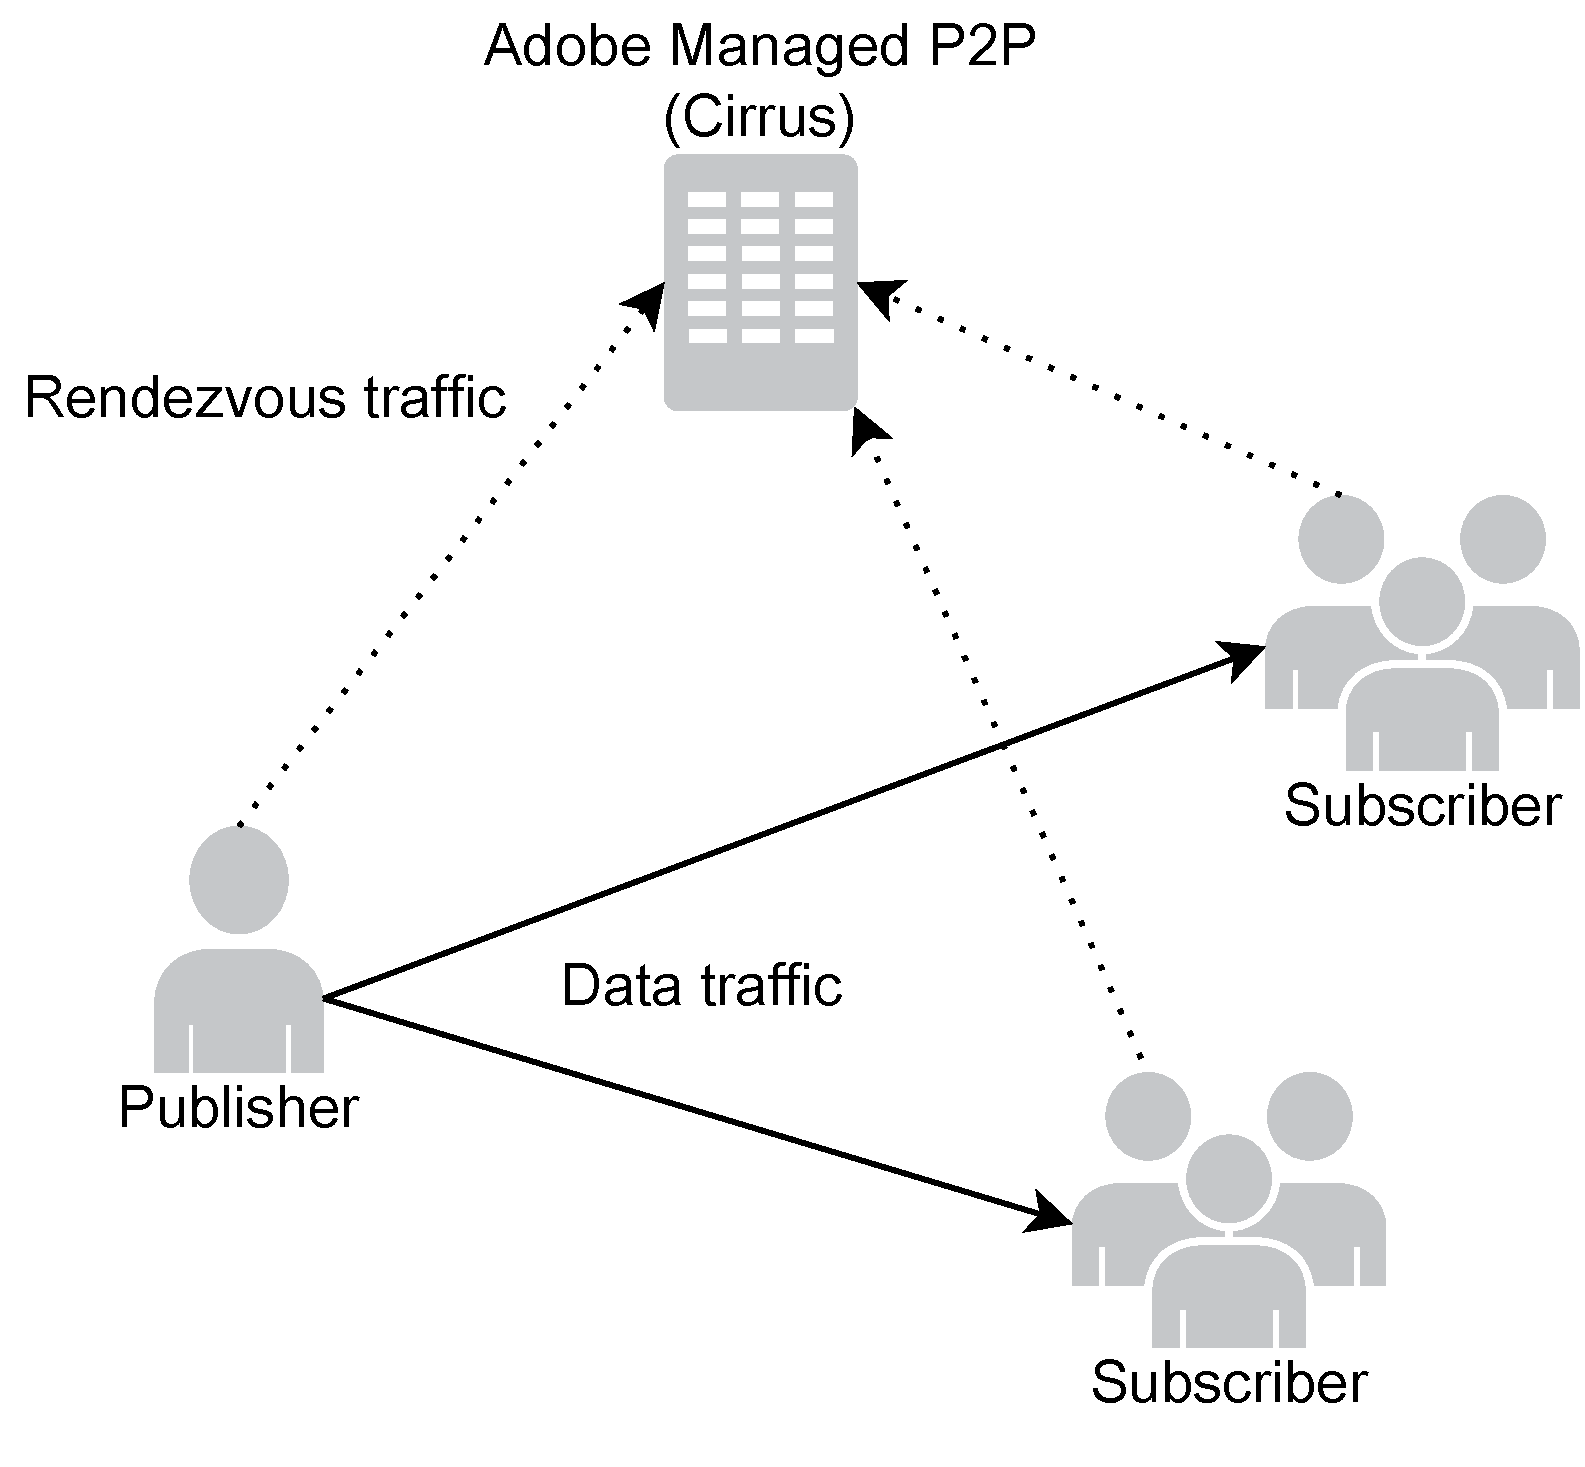
\includegraphics[scale=0.4]{./figures/cirrusAdobe.pdf}
      \caption[RTMFP architecture using Cirrus]{RTMFP architecture using Cirrus.}
	\label{fig:RTMFParchitecture}
\end{figure}
 
Some of the most valuable features is the possibility to easy integrate P2P multicast topologies where one source sends a video to a group of receivers.

\subsection{WebRTC}

WebRTC is part of the HTML5 proposal, it is defined in a W3C draft~\cite{webrtcW3cgroup}, and enables RTC capabilities between Internet browsers using simple JavaScript APIs. Providing video, audio and data P2P without any plugins. This API replaces the need of any plugin for P2P communications in browsers, WebRTC uses already existing standardized protocols, learned from SIP, to perform RTC. 

The project was open sourced by Google to keep working with the IETF in order to standardize the technology~\cite{haraldpublicWebRTC}.

WebRTC provides interoperability between different browser vendors, this allow the APIs to be accessible by the developers assuring high degree of compatibility (Figure~\ref{fig:marketshare}). Some of the major browsers that actively implement some of the WebRTC APIs are: Google Chrome, Mozilla Firefox and Opera. 

 \begin{figure}[h]
  \centering
    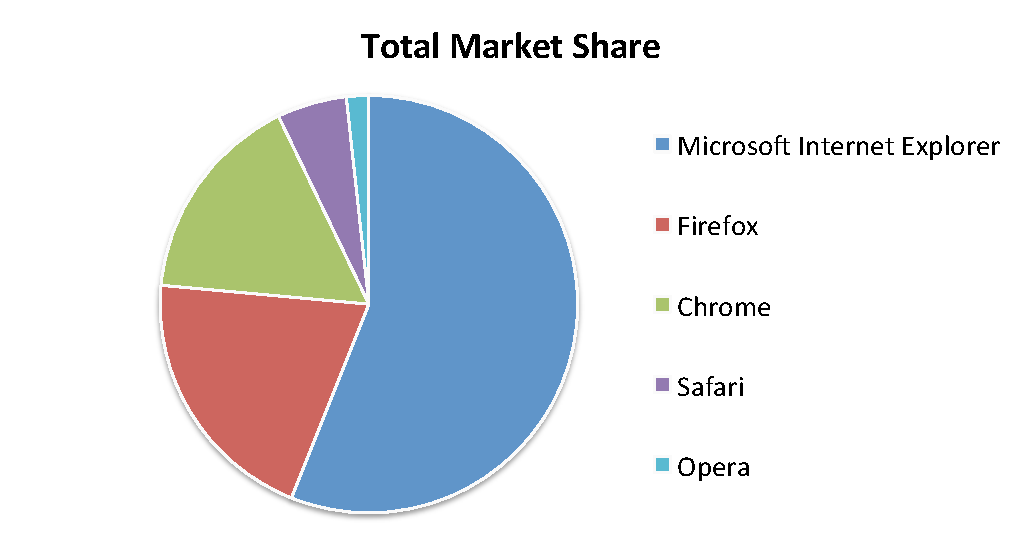
\includegraphics[width=1\textwidth]{./figures/marketshare}
      \caption[Market share of browser vendors by April 2013. Source~\cite{NetMarketShare}]{Market share of browser vendors by April 2013~\cite{NetMarketShare}.}
	\label{fig:marketshare}
\end{figure}

With WebRTC developers can provide applications for nearly half of the desktop devices available, mobile devices will integrate WebRTC as part of their HTML5 package to also enable RTC soon~\cite{ericssonbowser}.

WebRTC is composed by to important APIs that enable those features, GetUserMedia and PeerConnection. Both of them are accessible by JavaScript by the browser.
%It is able to solve NAT transversal environments by using a mixtures of ICE, TURN and STUN technologies. For the session description it uses a modified bundled version of SDP. The format used for packet transport is RTP and SRTP, modified WebSockets are in use for P2P DataChannel implementation to provide data transport multiplexed over the same stream. All the traffic is sent over UDP or TCP over the same port~\cite{alvestrandOverview2012}.
%
%WebRTC is part of the HTML5 package, both combined are an open cross-platform standard that aims to replace the Adobe proprietary proposal for P2P Real-Time Communication (RTC).
%
%By using HTML5 features we avoid the need of installing any extra software to be able to use real-time multimedia applications on the browser.

\subsubsection{Device Access API}
\label{sec:gum}

WebRTC uses an API called GetUserMedia to access media streams from local devices (video cameras and microphones). This API itself does not provide RTC, furthermore, provides media to be used as simple HTML elements in any web application. GetUserMedia allows developers to access local media devices using JavaScript code and generate media streams to be used either with the rest of the WebRTC APIs or with the HTML5 video element~\cite{getusermediaDraft}.

GetUserMedia is already interoperable between Google Chrome, Firefox and Opera~\cite{chromefirefoxinterop}.

This proposal was first attached directly to the WebRTC working group but has been published in a different draft, the usage of this API removes the need of using Adobe Flash to access the media device and also the plugin requirement.

 \begin{figure}[h]
  \centering
    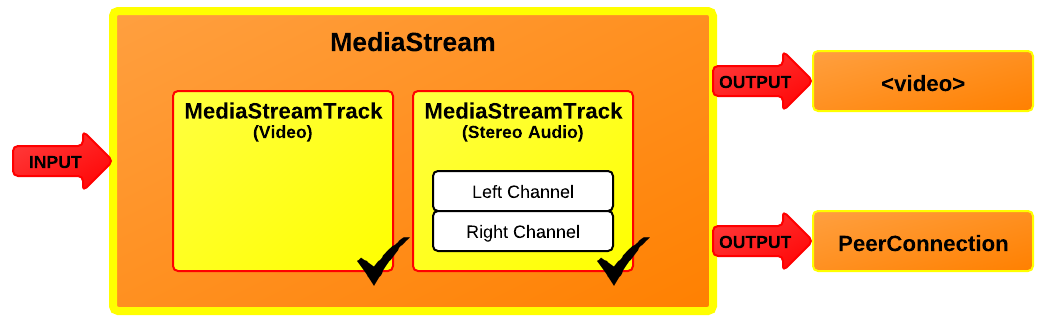
\includegraphics[scale=1]{./figures/mediastreamAPI.png}
      \caption[Media Stream API~\cite{getusermediaDraft}]{Media Stream API~\cite{getusermediaDraft}.}
	\label{fig:mediastreamAPI}
\end{figure}

Figure~\ref{fig:mediastreamAPI} illustrates how the browser access that media and the outputs delivered to the developer. We will use this function to build WebRTC enabled applications for RTC video conferencing. The video tag is an HTML5 a Document Object Model (DOM) \nomenclature{DOM}{Document Object Model} element that reproduces local and remote media streams.

GetUserMedia API works in a fallback model, this means than the JavaScript method will return an object that can be played in an HTML web application, a simple example of this method can be seen in the following code.

\lstset{language=JavaScript}
\begin{lstlisting}[caption=Simple example of video and audio access using JavaScript]
navigator.webkitGetUserMedia(cameraConstraints(), gotStream, function() {
	console.log("GetUserMedia failed");
});
    
function gotStream(stream) {
	console.log("GetUserMedia succeeded");
  	document.getElementById("local-video").src = webkitURL.createObjectURL(stream);
}
\end{lstlisting}

With the previous code, we are using the video and audio media from our devices to be played in an video HTML element identified as {\it local-video}. 

GetUserMedia also allow developers to set some specific constraints to the media acquisition. This help developers to better adapt the stream to their requirements, those {\it cameraConstraints()} are stored into a JavaScript Object Notation library and provided to the API through the {\it navigator.webkitGetUserMedia} method.

\subsubsection{Networking API}
\label{sec:pcAPI}

WebRTC uses a separate API to provide the networking support to transfer media to the other peers, this API is named {\it PeerConnection}~\cite{editorWebRTCdraft}. This API bundles all the internal mechanisms of the browser to enable media and data transfer, at the same time it also handles all the exchange signaling messages with specific JavaScript methods. 

Signaling will be exchanged using a topology similar to Figure~\ref{fig:webrtcExample} with the signaling being sent either by WebSockets or other HTTP polling protocols. Messages are built using a modified bundled version of SDP, WebRTC is similar to SIP as it can work over RTC and existing technologies.

WebRTC uses multiplexing over one port when sending the traffic, this means that media and data are sent over the same port from peer to peer, traffic is sent by UDP or TCP~\cite{alvestrandOverview2012}. This networking API provides signaling and NAT transversal techniques to bypass routers and firewalls, this part is very important to guarantee a high degree of success when establishing calls in different scenarios.

This P2P session establishment system works in a constrained environment similar to RTMFP but it has been designed to provide some degree of legacy for other SDP based technologies such as SIP. Figure~\ref{fig:webrtcExample} shows how a WebRTC simple P2P scenario works, the server used for signaling is a web server.

 \begin{figure}[h]
  \centering
    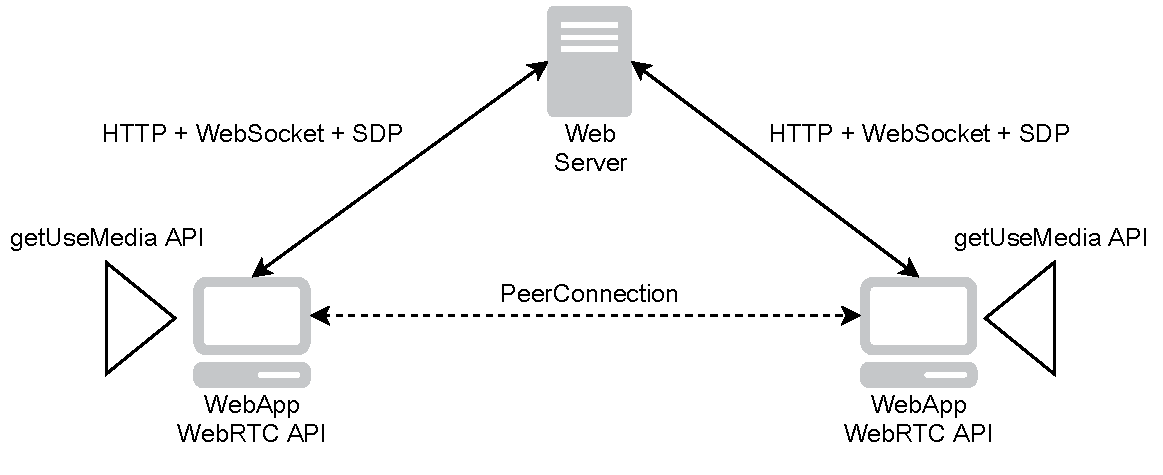
\includegraphics[width=1\textwidth]{./figures/webrtcExample.pdf}
      \caption[WebRTC simple topology for P2P communication]{WebRTC simple topology for P2P communication.}
	\label{fig:webrtcExample}
\end{figure}

Figure~\ref{fig:webrtcExample} does not show relay machines that provide NAT transversal solutions. In a real application we could host those relay machines either in the same web server or in external services, those servers must be introduced into the WebRTC {\it PeerConnection} configuration when starting a new call.

\lstset{language=JavaScript}
\begin{lstlisting}[caption=Simple example of {\it PeerConnection} using JavaScript]
pc = new webkitRTCPeerConnection(servers);
pc.onicecandidate = iceCallback1;

//Localstream is the local media obtained with the GetUserMedia API
pc.addStream(localstream);

function iceCallback1(event){
	if (event.candidate) {
		sendMessage(event.candidate);
	}
}

//When incoming candidate from the other peer we send it to the PeerConnection
pc.addIceCandidate(new RTCIceCandidate(event.candidate));

//This is fired when the remote media is received
pc.onaddstream = gotRemoteStream; 
function gotRemoteStream(e){
	document.getElementById("remote-video").src = URL.createObjectURL(e.stream);
}
\end{lstlisting}

Previous code describes a simple example on how to use the {\it PeerConnection} API to perform a P2P connection and start transferring media, this code works in conjunction with the code in section~\ref{sec:gum}. When building the new {\it PeerConnection} object we need to pass the JSON object {\it server} with the relay configuration for the NAT transversal process. 

\subsubsection{Control and Monitoring API}

Control and monitoring is an important part of all RTC protocols, this part is usually handled by the software that adapts the constraints and configurations to the available resources. 

In WebRTC, this is done through the Statistics Model and Constraints defined in the W3C draft~\cite{editorWebRTCdraft}, these methods are part of the actual {\it�PeerConnection} API defined in section~\ref{sec:pcAPI}. Once the {\it PeerConnection}�is made and media is flowing we need to measure the quality of the connection, this is done by retrieving the stats provided in the Real Time Control Protocol (RTCP) \nomenclature{RTCP}{Real Time Control Protocol} messages that are being sent over the link. 

To access this data contained on the control messages we need to call the {\it getStats()} method in the {\it PeerConnection}, this method will allow the developers to access that data in a JSON format that will require some post-processing. Statistical models will be useful for the developers to monitor the usage of their WebRTC applications and change the attributes of the {\it PeerConnection}.

With constraints developers are able to change media capture configuration by setting  Frames per Second (FPS) \nomenclature{FPS}{Frames per Second} and video resolution. Other attributes can be set on the {\it PeerConnection} such as bandwidth requirements, transfer rate is automatically adjusted in WebRTC using its internal mechanisms but we can set a maximum value. 

JSON objects for camera and bandwidth constraints must be defined as in the following code.

\lstset{language=JavaScript}
\begin{lstlisting}[caption=JSON objects for constraints attributes in WebRTC]
//Media constraints
var constraints = {
	"audio": true,
 	"video": {
  		"mandatory": {
   			"minWidth": "300",
   			"maxWidth": "640",
   			"minHeight": "200",
   			"maxHeight": "480",
   			"minFrameRate": "30"
  		},
  	"optional": []
 	}
}

//Bandwidth
var pc_constraints = {
	"mandatory": {},
 	"optional": [
 	 {
   		"bandwidth": "1000"
  	}
 	]
}
\end{lstlisting}

Both constraints objects are added to the {\it GetUserMedia} and {\it PeerConnection} methods when building the new object. Values are in pixels for the media attributes and Kbit/s for the rate configuration.

\subsubsection{Low vs High level API}

During the development of WebRTC there has been a lot of discussion in the different working groups about the API layout, those APIs have been designed using the feedback provided by the developers and experts on the area.

One of the difficult parts in the standardization process has been to decide the complexity level of the API, how much is available to be accessed by the developers and which configurations or mechanisms should be automatized in the browser. After long discussion, WebRTC is now working with JavaScript Session Establishment Protocol (JSEP) \nomenclature{JSEP}{JavaScript Session Establishment Protocol}~\cite{jsepIETF}, this API is a low level API that gives the developers control of the signaling plane allowing each application to be used in different environments, some will give legacy to SIP or Jingle protocols meanwhile others might only work in a closed web domain. 

The media process is done in the browser but most of the signaling is handled in the JavaScript plane by using JSEP methods and functions. Figure~\ref{fig:JSEP} represents the JSEP signaling model, this system extracts the signaling part leaving media transmission to the browser. However, JSEP provides mechanisms to create offers and answers, as well to apply them to a session. The way those messages are communicated to the remote side is left entirely up to the application.

One interesting feature that JSEP provides is called {\it rehydration}, this process is used whenever a page that contains an existing WebRTC session is reloaded keeping the existing session alive. This will help to avoid session cuts when accidentally reloading the page or with any automatic update from the web application. With {\it rehydration} the current signaling state is stored somewhere outside the page, either on the server or in browser local storage~\cite{jsepIETF}.
 
 \begin{figure}[h]
  \centering
    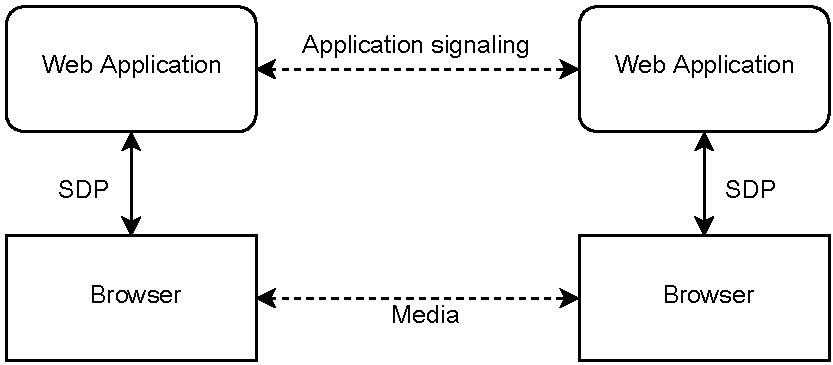
\includegraphics[scale=0.9]{./figures/JSEP.pdf}
      \caption[JSEP signaling model]{JSEP signaling model.}
	\label{fig:JSEP}
\end{figure}

Low level APIs allow developers to build their own high level APIs that handle all the WebRTC protocol from media access to signaling. Those high level methods are useful to simplify the way JavaScript developers use their applications, building object oriented calls we can have JavaScript libraries that set up and maintain multiple calls at the same time. The benefits of having low level JSEP API for WebRTC are the multiple possibilities to adapt WebRTC to the requirements of each specific application.

In this thesis we will be using some high level APIs that handle signaling over WebSockets and statistics.

\subsubsection{Internals of WebRTC}

WebRTC has multiple internal mechanisms to enable the RTC on the browser level by APIs. Those mechanisms work together to accomplish all the needs for WebRTC features, some of them are related to the network level or video acquisition.

One of WebRTC main issues is NAT transversal, this problem will affect all RTC technologies. Real-time P2P protocols cannot success in all environments without a NAT transversal solution, in SIP and WebRTC this problem is addressed with the usage of Simple Transversal Utilities for NAT (STUN) \nomenclature{STUN}{Simple Transversal Utilities for NAT} and Traversal Using Relays around NAT (TURN) \nomenclature{TURN}{Traversal Using Relays around NAT}~\cite{stunIETF}~\cite{turnIETF}. Both of these methods are combined with Interactive Connectivity Establishment (ICE) \nomenclature{ICE}{Interactive Connectivity Establishment} technique that helps WebRTC to decide which is the best way to bypass NATs and firewalls, ICE is widely used in P2P media communications and has proven to be reliable when choosing the best option to succeed with the connexion~\cite{iceIETF}.

TURN and STUN machines are usually placed outside the local network of the clients and help them to find the way to communicate each other by discovering new open paths, the final decision is taken by the ICE mechanism in WebRTC. STUN server provide different IP and port configurations that allow a direct connection to the peer behind the firewall, those configurations are named {\it candidates}, this information is given to the sender that process the information and tries to choose the best {\it candidate}. On the other side, TURN works as a relay, this option should be always stated as the last resort when there is no valid {\it candidate} for connectivity. TURNs will reroute there traffic from one peer tot the other. 

All traffic in WebRTC is done over UDP except the case of TURN TCP and multiplexed over the same port.

Media encoding in WebRTC is done through codecs implemented in the browser internals, those codecs are decided in the IETF working group and have been discussed for long time.

Defined codecs for audio are G711 and Opus. G711 is an International Telecommunication Union (ITU) \nomenclature{ITU}{International Telecommunication Union} standard audio codec that has been used in multiple real time applications such as SIP. In real-time media applications Opus is also a good alternative for G711, Opus is a lossy audio compression format codec developed by the IETF and that is designed to work in real-time media applications on the Internet~\cite{opusIETF}. Opus can be easily adjusted for high and low encoding rates being a good candidate for the needs of WebRTC.

Along with the codecs, the audio engine for WebRTC also includes some interesting mechanisms such as Acoustic Echo Canceler (AEC) \nomenclature{AEC}{Acoustic Echo Canceler} and Noise Reduction (NR) \nomenclature{NR}{Noise Reduction}. The first mechanism is a software based signal processing component that removes, in real time, the acoustic echo resulting from the voice being played out coming into the microphone, with this, WebRTC avoids to create audio loops with the output and input sound devices of computers. NR is a component that removes background noise associated to real time audio communications. 

Those mechanisms provide a smooth audio input for WebRTC protocol.

There has been a lot of discussion regarding video codec, two of the proposed codecs are H.264 and VP8. H.264 is a standard codec for video compression, this codec is widely used for recording and transmission of high definition video. Originally it was also selected due its high compatibility with existing devices and software, H.264 has made some controversy as it is patented and licensed by MPEG LA and may add some patenting problem for WebRTC. VP8 is a video compression codec owned by Google released in May 2010, VP8 is supported by Chrome, Opera and Firefox by default and is the de facto codec for WebRTC by May 2013. Later on, Google announced a VP8 patent cross-license agreement to provide royalty-free license to allow developers to implement VP8 video in their web applications~\cite{vp8Google}. This video codec is adaptive and performs well in low bandwidth links at the same time as providing royalty-free implementation.

WebRTC is not only useful for sending media, it can also provide P2P data transfer. This feature is named {\it Data Channel} and provides real time data transfer, this can be used with multiple purposes, from real time IM service to gaming, but it is interesting to as {\it Data Channel} allows generic data exchange in a bidirectional way between two peers~\cite{datachanIETF}. Non-media data type in WebRTC is handled by using System Control Transmission Protocol (SCTP) \nomenclature{SCTP}{System Control Transmission Protocol} encapsulated over Datagram Transport Layer Security (DTLS) \nomenclature{DTLS}{Datagram Transport Layer Security}~\cite{sctpIETF}~\cite{dtlsIETF}~\cite{datachanIETF}. 

The encapsulation of SCTP over DTLS on top of ICE/UDP provides a NAT traversal solution that combines confidentiality, source authentication and integrity with protected transfers. This data transport service can operate in parallel with media transfer and is sent multiplexed over the same port. This feature of WebRTC is accessible from the JavaScript {\it PeerConnection} API by a combination of methods, functions and callbacks. From the developer perspective all the previous statements regarding security and transport are made in the browser internals providing a simple and reliable way of sending P2P secure data over WebRTC.

WebRTC provides Secure Real-time Transport Protocol (SRTP) \nomenclature{SRTP}{Secure Real-time Transport Protocol} to allow media to be secured.

Quality of Service (QoS) \nomenclature{QoS}{Quality of Service} for WebRTC is also being discussed in the IETF and a draft is available with some proposals~\cite{qosWebRTCIETF}. WebRTC uses DiffServ packet marking for QoS but this is not sufficient to help prevent congestion in some environments. When using DiffServ the problem arises from the Internet Service Providers (ISPs) as they might be using their own packet marking with different DiffServ code-points, those won't be interoperability between ISPs, there is an ongoing proposal to build consistent code-points. Audio/video packets will be marked as priority using DSCP mappings with audio being more important than video or data~\cite{qosWebRTCIETF}. 

WebRTC also uses a Google congestion control algorithm that enables proper congestion control mechanisms for rate adaptation~\cite{alvestrandCongestion2012}. The aim of this algorithm is to provide performance and bandwidth sharing with other ongoing conferences and applications that share the same link.
%\subsection{Support}
%The following companies and organizations have supported and are actively working in the development of WebRTC standard in the W3C: Google, Mozilla and Opera~\cite{googleAnnouncement}. Other companies such as Microsoft have supported browser-to-browser solution but have published their own proposal which differs with the one published in the WebRTC WG, called CU-RTC-Web~\cite{curtcweb} which is a lower level API that claims to do everything that JSEP does.
%
%During the firsts attempts to build a reliable solution for WebRTC Ericsson Labs presented an initial API based on the preliminary work done in the WHATWG, this API was called ConnectionPeer API and required an special module to be installed in your browser~\cite{ericssonwebrtc}. Ericsson lately dropped from the effort to build it's own browser to focus in the standardization and codec discussion, leaving the API implementation to the Mozilla and Chrome teams. The original API evolved rapidly during the next months thanks to the WGs and the developer community feedback that is experimenting with the unstable API.
%
%%\subsection{Milestones}
%During the process of standardization some important moments should be remarked. In January 2012 Opera implemented the first version of WebRTC getUserMedia for accessing the camera and audio~\cite{operaannouncement}, during this year getUserMedia is available in the stable version of Opera. 
%
%Google Chrome integrated the first version of WebRTC in its DEV and Canary channels of the browser during January 2012~\cite{chromeannouncement}, in June 2012 it started moving its API to the stable channel hidden behind a flag, in November 2012 WebRTC becomes fully available in Google Chrome stable channel and is open for public usage~\cite{chromestable}. 
%
%Mozilla Firefox started working on the getUserMedia implementation early 2012 delivering the first version of media access trough API at the beginning of 2012 in the alpha version~\cite{mozillablog}, in April 2012 Mozilla published a WebRTC video demo running on Firefox in the "adler" channel~\cite{mozillawebrtc}, also supporting some primitive DataChannel API. Later in October Firefox Nightly was carrying the first unstable version of the WebRTC API including DataChannel~\cite{mozillafinal}, Mozilla announced in September 2012 that the stable version of WebRTC will be shipped along with Firefox 18 in January 2013~\cite{mozillacomming}, finally, the first public announcement of interoperability between Firefox and Chrome was done the 4th of February 2013~\cite{chromefirefoxinterop}.
%
%Some announcements done from Microsoft point out that they are also working in some implementation into Internet Explorer by using CU-RTC-Web as the default standard, at the moment only the Media API information is publicly available~\cite{microsoftcapture}.
%
%In October 2012 Ericsson announced the world's first WebRTC-enabled browser for mobile devices called "Bowser" with support for iOS and Android, this browser is able to handle WebRTC calls using RTCWeb Offer/Answer Protocol (ROAP) which is an old discontinued version of the WebRTC API that has moved to Javascript Session Establishment Protocol (JSEP). This browser also differs from the previous desktop alternatives on the codec side, it is carrying H.264 for video and G.711 for audio~\cite{ericssonbowser}. The API provided by Bowser is not fully W3C compliant.

%\subsection{Issues in WebRTC}
%
%WebRTC uses a mixture of different technologies to perform peer-to-peer communication between clients, those technologies range from SRTP, RTP, RTCP and multiple codecs that are being discussed. This scenario makes performance the key point for success in developing stable WebRTC applications. 
%
%Performance is manly related to computer capabilities and the ability to encode/decode at the same time as transferring and monitoring multiple peer connections. All those tasks are run over the browser and not directly on the OS, this is good for interoperability between platforms but bad in the performance aspect. Compared to Adobe technologies which uses a plugin, the performance they can deliver should be higher as they do not use as many application layers.
%
%Media applications are delay sensitive and require a low packet loss for its proper function, WebRTC is working on this aspect by trying to implement congestion control over the connection stablished between peers, this work is not completed yet and will arise as a problem in the near future. Packet loss due to system capacity and bandwidth are measurable in WebRTC using the Stats API, this API provides information about the PeerConnection performance and is accessible by JavaScript.
%
%Media constraints and bandwidth statistics will make a big difference in how media is acquired in WebRTC. Browsers and web applications have always tolerate some amount of delay and packet losses but this is not possible in media infrastructures for real time applications, an effort is needed to handle Quality of Service (QoS) in WebRTC to compete with RTMFP.

%\subsubsection{Quality of Service}
%
%Quality of Service (QoS) for WebRTC is being discussed and an internet draft is available with some proposals~\cite{qosWebRTCIETF}. WebRTC uses DiffServ packet marking for QoS but this is not sufficient to help prevent congestion in some environments. When using DiffServ the problem arises from the Internet Service Providers (ISPs) as they might be using their own packet marking with different DiffServ code-points, those won't be interoperability between ISPs, there is an ongoing proposal to build consistent code-points. Audio/video packets will be marked as priority using DSCP mappings with audio being more important than video or data~\cite{qosWebRTCIETF}. 
%
%The possibility to combine QoS in the transport layer with the constraints and stats of the WebRTC API will help developers to build more adaptive applications, for example, lowing the Frames per Second (FPS) in the case of high packet losses will reduce the bandwidth usage in the case of congestion of the link. This is possible thanks to the Stats API that provide the data statistics for the peer connection.
%
%Some environments will also require better QoS as their bandwidth will be lower, examples in the use case draft relate this to surveillance cameras or similar approaches~\cite{WebRTCcasesIETF}. In these cases QoS should be modified by using the API, this situation can lead also to malicious JavaScript injection that could flood the path with packets. 

\subsubsection{Security concerns}

To handle the signaling in WebRTC we use a web server, this web server will exchange the message between the peers in multiple different ways. Even this system provides high flexibility for developers to allow multiple scenarios, it also has some important security concerns~\cite{WebRTCcasesIETF}. Figure~\ref{fig:webrtcExample} represents the simple topology for a WebRTC call, web server relays the signaling messages to the peers and the media transport is done between them and handled by the browser.

Obviously, this system poses a range of new security and privacy challenges different from traditional VoIP systems. It has to avoid malicious calling or having a call established without user knowledge, considering that those APIs are able to bypass Firewalls and NAT, Denial of Services (DoS) \nomenclature{DoS}{Denial of Service} attacks can also become a threat.

Actual browsers execute JavaScript scripts provided by the accessed web sites, this also includes malicious scripts, but in the case of WebRTC this points out some privacy problems. In a WebRTC environment we consider the browser to be a trusted unit and the JavaScript provided by the server to be unknown as it can execute a variety of actions in the browser. At minimum, it must not be possible for arbitrary sites to initiate calls to arbitrary locations without user consent~\cite{rtcwebSecurityIETF}. To approach this, the user must make the decision to allow a call (and the access to its webcam media) with previous knowledge of who is requesting the access, where the media is going or both.

In web services, issues such as Cross-site scripting (XSS) \nomenclature{XSS}{Cross-site scripting} provide high risk of privacy vulnerability. Those situations, shown in Figure~\ref{fig:xss} are given when a third-party server provides JavaScript scripts to a different domain, this script cannot be trusted by the original domain that the user is accessing and could trigger browser actions that could harm the privacy. For example, in WebRTC, we could load a malicious script from a third-party entity that builds a WebRTC call to an undesired receiver without the user noticing this problem. Nowadays, browsers provide some degree of protection against XSS and do not let some scripting actions to be performed.

Other related vulnerabilities in WebRTC APIs is the possibility to establish media forwarding to a third peer, for example, once the user has accepted the access to the media the provided JavaScript will build one {\it PeerConnection} to the receiver and one to a remote server that could store the call without the user noticing. Those problems are not only related to WebRTC and could be given in related protocols.

 \begin{figure}[h]
  \centering
    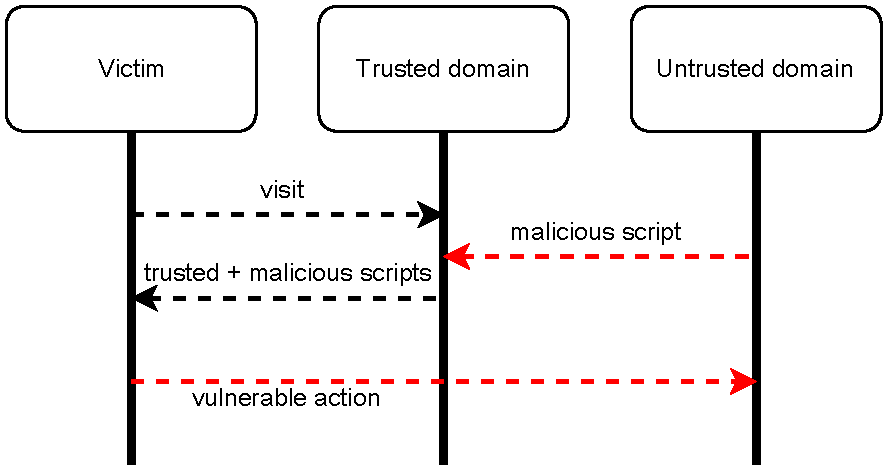
\includegraphics[scale=0.9]{./figures/xss.pdf}
      \caption[Example of cross-site scripting attack]{Example of cross-site scripting attack.}
	\label{fig:xss}
\end{figure}

WebRTC calling procedure is done by the JavaScript provided by the server, this is a security issue as the user must trust an unknown authority server. Calling services commonly use Hypertext Transfer Protocol Secure (HTTPS) \nomenclature{HTTPS}{Hypertext Transfer Protocol Secure} for authentication whose origin can be verified and users should be verified cryptographically (DTLS-SRTP). Browser peers should be authorized before starting the media flow, even this can be done by the {\it PeerConnection} itself using some Identity Provider (IdP) that supports OpenID or BrowserID to demonstrate their identity~\cite{rtcwebSecurityArchIETF}. Usually this problem is not particularly important in a closed domain, cases where both peers are in the same social network and provide their profiles to the system and those are exchanged previous to the call, but it arises as a big issue when having federated calls from different domains such in Figure~\ref{fig:idpWebRTCcall}.

 \begin{figure}[h]
  \centering
    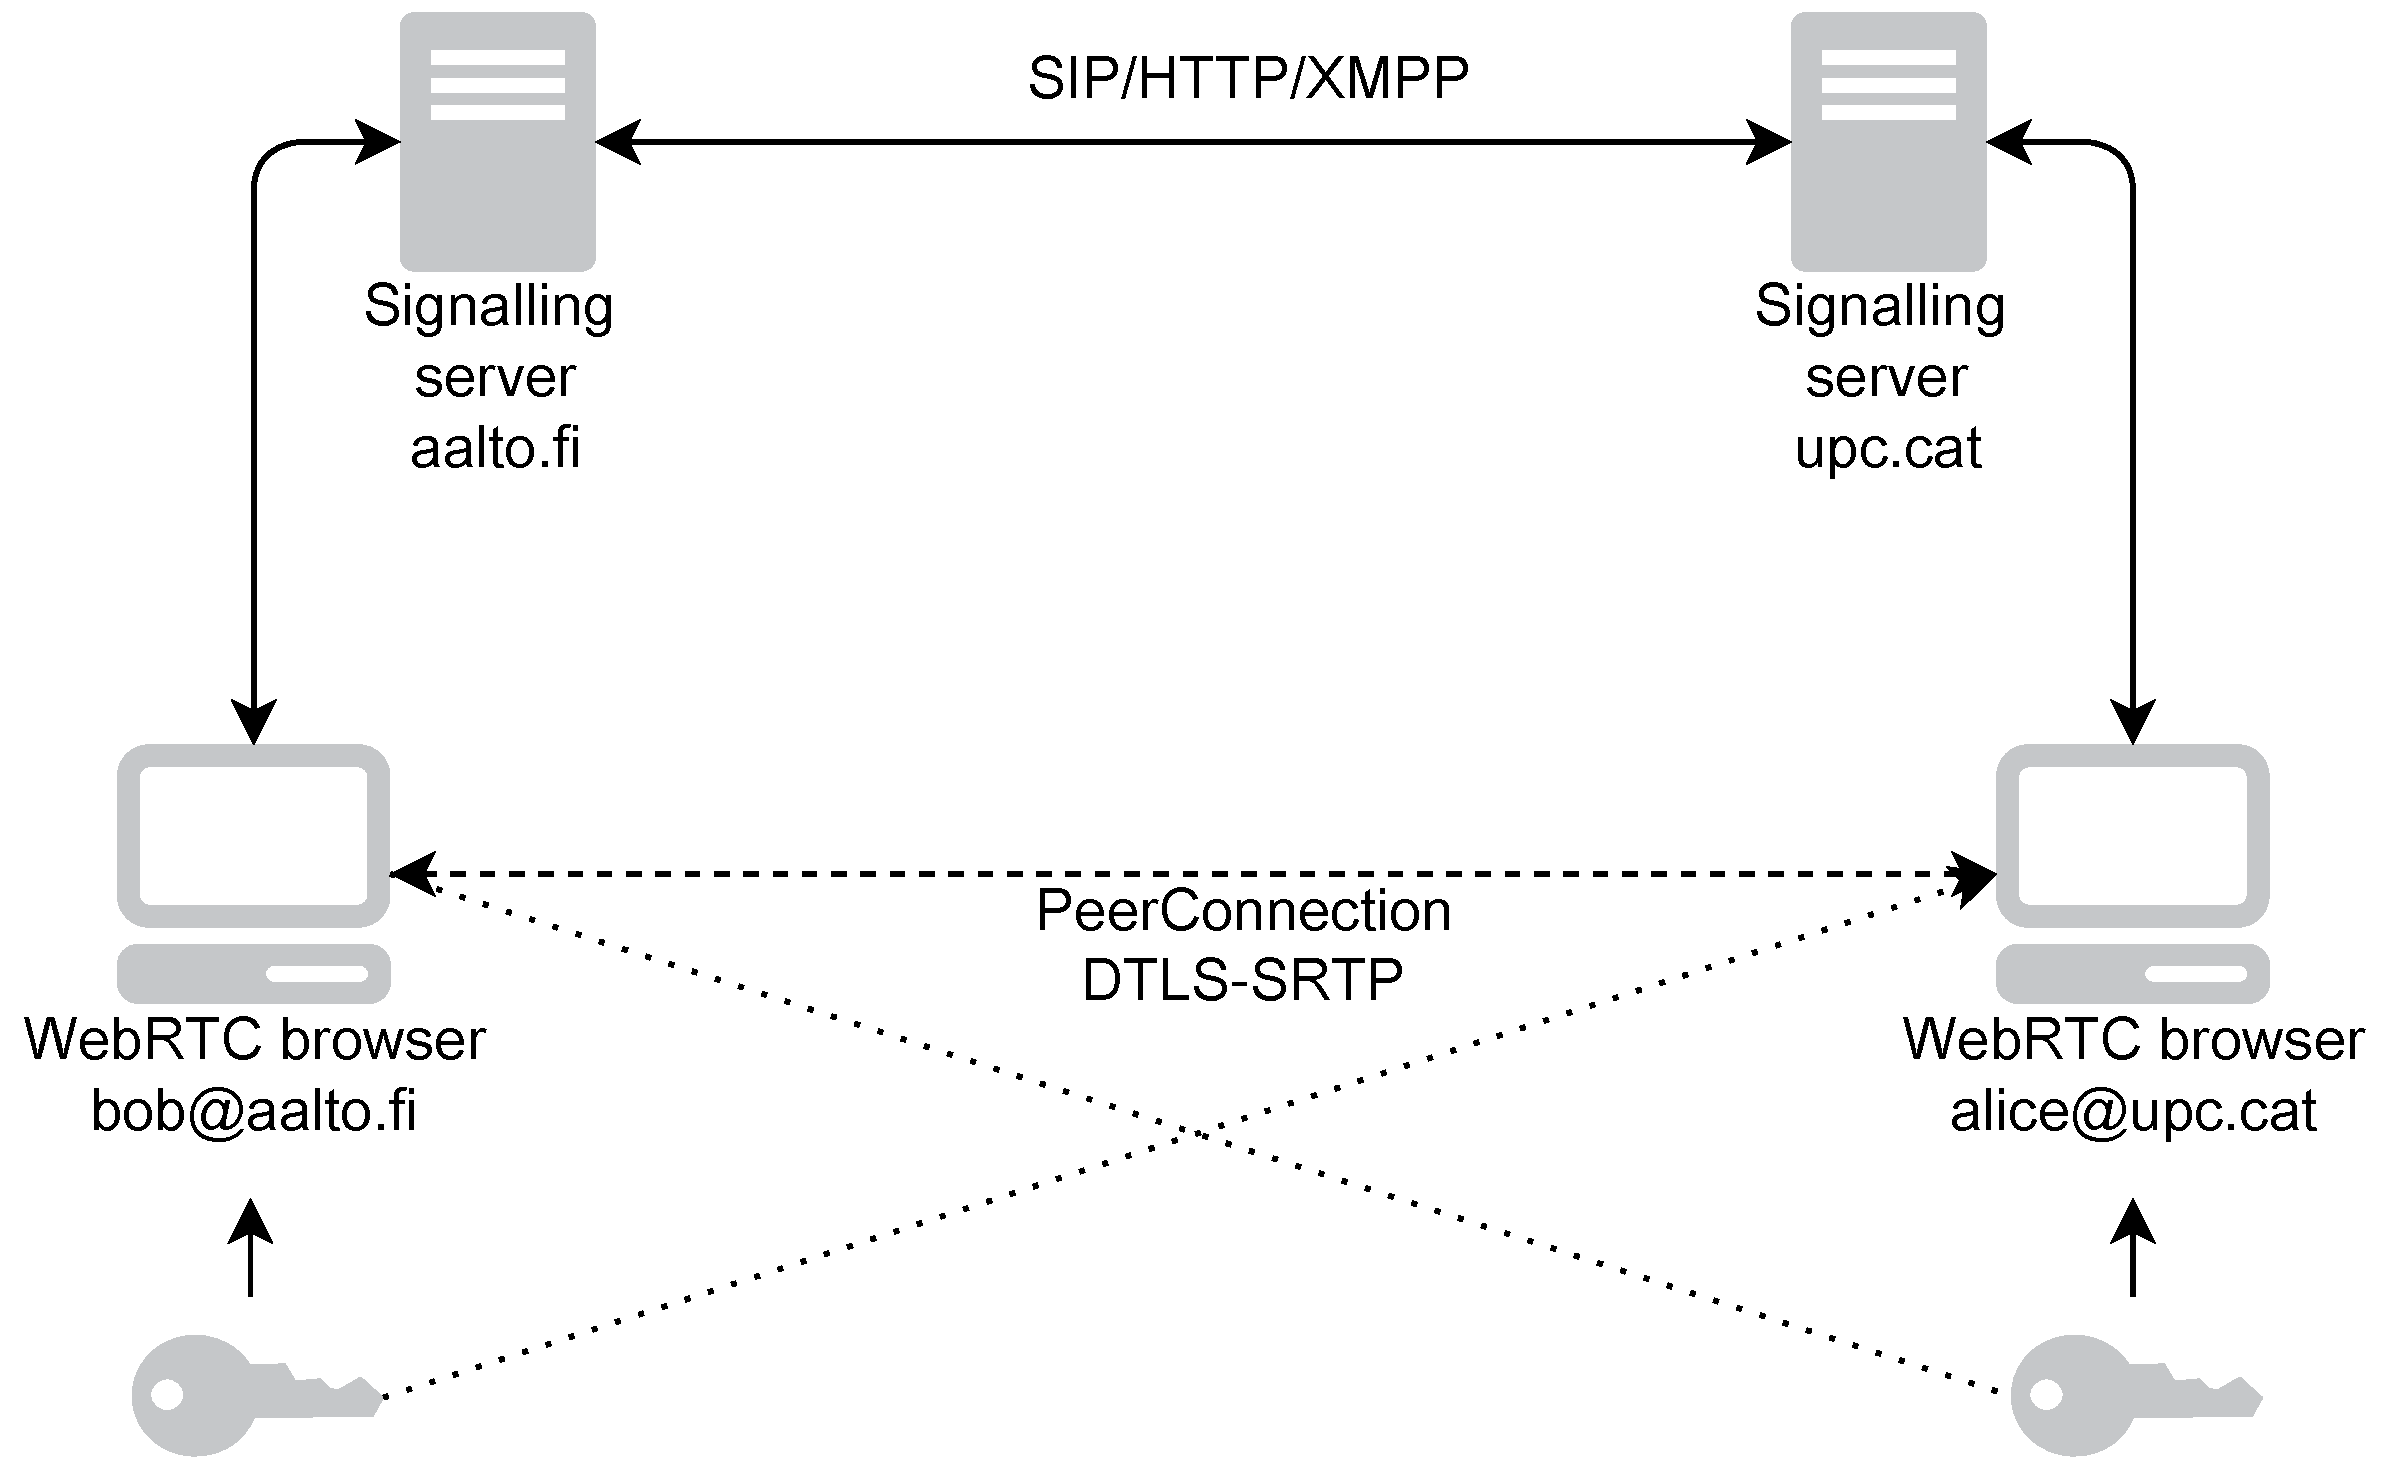
\includegraphics[width=1\textwidth]{./figures/idpWebRTCcall.pdf}
      \caption[WebRTC cross-domain call with Identity Provider authentication]{WebRTC cross-domain call with Identity Provider authentication.}
	\label{fig:idpWebRTCcall}
\end{figure}

If the web service is running over a trusted HTTPS certificate and has been authorized access to the media will be automatically after the first time, otherwise, the user will have to verify the access each time. Once the media is acquired the actual API builds the ICE candidates for media verification. Authentication and verification in WebRTC is an ongoing discussion in the working groups.

Security an privacy issues in WebRTC can be given in multiple layers of the protocol, the increment of trust for the provider gives some vulnerability issues that sometimes cannot be easily solved if the aim is to keep a flexible and open sourced real time protocol. Some use cases for WebRTC also incorporate some level of vulnerability as the JavaScript will be provided by a third-party and could led to privacy vulnerability, in the use case of media streaming, advertisement or call centers those providers could pick data form the users and store them for further usage~\cite{WebRTCcasesIETF}.

\subsection{Comparison of WebRTC, SIP and RTMFP}

After describing various RTC mechanisms and all the similar alternatives for WebRTC, Table~\ref{fig:CompareRTC} is a summary of common features between SIP, RTMFP and WebRTC. In this Table~\ref{fig:CompareRTC}, common internal mechanisms are described for all of them.

RTFMP is a proprietary protocol which mean that might have its own mechanisms other than the standardized ones stated on the table to solve some of the issues.

All there protocols are designed to provide the same real time functionalities but in different ways, meanwhile SIP is a protocol that helped to develop some of the important mechanisms that will be used in other technologies is still not easily accessible by developers. On the other side, RTMFP provides real time communication for developers in a licensed way having some of their mechanisms not standardized and with compatibility issues.

From the mobile perspective, SIP is used in mobile technology and WebRTC has announced to be compatible with near versions of iOS and Android~\cite{ericssonbowser}. Furthermore, RTMFP has active support for Android but is still not able to extend its usage to iOS platforms.

All three protocols provide NAT traversal solutions but RTMFP is the only one that provides a proprietary solution that is not standardized, SIP and WebRTC use a conjunction of TURN, STUN and ICE mechanisms.

\begin{table}[h]
\begin{center}
	\begin{tabular}{| l | c | c | c |}
	\hline
    	 & SIP & RTMFP & WebRTC \\ \hline
    	Plugin-enabled & No &Yes & No \\ \hline
    	Cross-domain & Yes & No & No \\ \hline
    	Licensed & No & Yes & No \\ \hline
    	Mobile & Yes & Partially & Yes \\ \hline
    	Audio & Yes & Yes & Yes \\ \hline
    	Video & Yes & Yes & Yes \\ \hline
    	Data & No & No & Yes \\ \hline
	\hline \hline
	TURN & Yes & No & Yes \\ \hline
    	STUN & Yes & No & Yes \\ \hline
    	SDP & Yes & No & Yes \\ \hline
    	RTP & Yes & No & Yes \\ \hline
    	SRTP & Yes & No & Yes \\ \hline
    	UDP & Yes & Yes & Yes \\ \hline
    	TCP & No & No & Yes \\ \hline
    	SCTP & No & No & Yes \\ \hline
	\hline \hline
    	VP8 & No & No & Yes \\ \hline
    	H.264 & Yes & No & Yes \\ \hline
    	G711 & Yes & No & Yes \\ \hline
    	Opus & No & No & Yes \\
	\hline
	\end{tabular}
      \caption[Feature comparison between SIP, RTMFP and WebRTC]{Feature comparison between SIP, RTMFP and WebRTC.}
	\label{fig:CompareRTC}
\end{center}
\end{table}
	
All of them are valid options, in this thesis we will work with WebRTC and its related mechanisms,
	
